\chapter{Introduction and theory}
\label{chap:theory}
In order to describe the search for invisible decays of the Higgs boson (``Higgs to invisible''), it is necessary to describe the theory behind them and the statistical techniques used in carrying out the search. This chapter will start with an introduction to the current best theory of particle physics, the \ac{SM}, focusing on the Higgs mechanism, before outlining the motivations behind, and some candidates for, physics \ac{BSM}, then concluding with a discussion of the statistics of hypothesis testing. Natural units, where $\hbar=c=1$, Einstein summation convention and Feynman slash notation are used throughout. Four vector indices are labeled using Greek letters, and gauge group generators using roman letters.

%??CHECK PLOT AXIS LABEL SIZES AND THAT LEGEND TERMS ARE STANDARD OR IN TEXT

\section{The standard model of particle physics}
\label{sec:SM}
The SM describes the interaction of the particles currently thought to be fundamental with the strong, weak and electromagnetic forces~\cite{GlashowPartialSymmetries,WeinbergModelOfLeptons,SalamNobelSymposium,eightfoldway}. Its predictions, which come from specifying the symmetries the theory respects and how they are broken, the particles in the theory, and 18 free parameters, have been tested in many different experiments, in some cases up to one part in a trillion \cite{PhysRevLett.100.120801}. However, it does face challenges, one example being that it does not describe \ac{DM}. 

The SM is a gauge invariant \ac{QFT}. To construct a QFT the symmetries that are respected by the theory and the fields it describes must be specified. The symmetries are important because of Noether's theorem, which states that for every continuously differentiable symmetry of the Lagrangian of a theory there is a corresponding conservation law~\cite{Noether:1918zz,doi:10.1080/00411457108231446}. An example of this is Poincar\'e invariance, the invariance of the laws of physics under translations and rotations in space and time, which leads through Noether's theorem to the conservation of energy, linear momentum and angular momentum. In addition to giving rise to conservation laws, some types of symmetry lead to additional fields being required to preserve invariance, this will be discussed further in \SectionRef{sec:gaugesym} \cite{PhysRev.96.191}.

Because particles correspond to the quantised excitations of fields, the fields that can be described by the QFT are constrained by the fundamental particles seen in nature. In order to add a new field an explanation for why the corresponding particle has not yet been observed must, therefore, be provided. Specifically, a scalar field corresponds to a spin zero boson, spinor fields correspond to spin half fermions, and vector fields correspond to spin 1 bosons. We will now go through the particles observed in nature and how they are represented in the SM.

\subsection{Fundamental particles in nature}
There are two types of fundamental particles in nature, fermions and bosons. The fermions observed in nature that are currently thought to be fundamental are then divided into those which interact via the strong nuclear force (the quarks), and those which don't (the leptons). Both the quarks and leptons have two further types: charged and neutral in the case of the leptons, and up type and down type in the case of the fermions. Another interesting feature of the fermions is that they are arranged in three generations. Each generation has one fermion of each type with the same quantum numbers as those in the other generations, except that the mass is different. \TableRef{tab:fermions} shows this structure.

\begin{table}
  \caption{The fundamental fermions observed in nature separated into their three generations. Each particle shown also has an antiparticle with opposite charge and identical mass. Values taken from~\cite{Agashe:2014kda}}
  \label{tab:fermions}
  \begin{tabular}{ccccccc}
  \hhline{=======}
  &\multicolumn{3}{|c|}{Leptons}& \multicolumn{3}{c}{Hadrons} \\
  \cline{2-7}
  Generation & \multicolumn{1}{|c}{Particle} & Mass & \multicolumn{1}{c|}{Electric Charge} & Particle & Mass & Electric Charge \\
  \hhline{=======}
  \multirow{2}{*}{1} & \Pem & 511 \keV & -1 & \Pqu & 2.3 \MeV & $+\frac{2}{3}$ \\
  & \Pgne & $\sim$0 & 0 & \Pqd & 4.8 \MeV & $-\frac{1}{3}$ \\
  \hline
  \multirow{2}{*}{2} & \Pgmm & 105.7 \MeV & -1 & \Pqc & 1.275 \GeV & $+\frac{2}{3}$ \\
  & \Pgngm & $\sim$0 & 0 & \Pqs & 95 \MeV & $-\frac{1}{3}$ \\
  \hline
  \multirow{3}{*}{2} & \Pgtm & 1.777 \GeV & -1 & \Pqt & 173.2 \GeV & $+\frac{2}{3}$ \\
  & \Pgngt & $\sim$0 & 0 & \Pqb & 4.18 \GeV & $-\frac{1}{3}$ \\
  \hhline{=======}
  \end{tabular}
\end{table}

The bosons in nature also have two types. The first type are vector bosons, which mediate the three fundamental interactions described by the SM. The vector bosons are summarised in \TableRef{tab:bosons}, where it can be seen that their masses are very different, the photon and the eight gluons being massless, while the \PWpm and \PZ bosons are massive. As we will see in \SectionRef{sec:ssb}, explaining these masses requires the Higgs mechanism~\cite{Englert:1964et,Higgs:1964ia,Higgs:1964pj,Guralnik:1964eu,Higgs:1966ev,Kibble:1967sv}. The Higgs mechanism also gives rise to the other type of boson seen in nature, the scalar Higgs boson. In order to see how all of the above particles are represented in the SM, an introduction to gauge theories is necessary.

\begin{table}
  \caption{The fundamental vector bosons observed in nature separated by the force which they mediate. Values taken from~\cite{Agashe:2014kda}.}
  \label{tab:bosons}
  \begin{tabular}{lccc}
    \hline
    \hline
    Force & Particle & Mass & Electric Charge \\
    \hhline{====}
    Electromagnetism & \Pgg & 0 & 0 \\
    \hline
    \multirow{2}{*}{Weak} & \PWpm & 80.4 \GeV & $\pm 1$ \\
    \cline{2-4}
    & \PZ & 91.2 \GeV & 0 \\
    \hline
    Strong & g & 0 & 0 \\
    \hline
    \hline
  \end{tabular}
\end{table}

\subsection{Introduction to gauge theories}
\label{sec:gaugesym}
Gauge symmetries are local transformations, i.e. the transformation can be different at different points in space and time, that form a symmetry group. To see the effect of imposing such a symmetry on a theory, consider imposing local invariance under U(1) transformations on the Dirac Lagrangian for a fermion, $\psi$, with mass, $m$:
\begin{equation}
  \label{eq:globaldiraclagrangian}
  \mathcal{L}=i\bar{\psi}\slashed{\partial}\psi-m\bar{\psi}\psi~\cite{griffiths2008introduction}.
\end{equation}

This Lagrangian is invariant under a global $U(1)$ transformation $\psi\rightarrow e^{iq\theta}\psi$, where q and $\theta$ are constant. However, if the $U(1)$ transformation is local i.e. $\theta$ is a function of spacetime position the Lagrangian is no longer invariant and transforms as:
\begin{equation}
  \label{eq:gaugeviolating}
  \mathcal{L}\rightarrow\mathcal{L}-q(\partial_{\mu}\theta)\bar{\psi}\gamma^{\mu}\psi.
\end{equation}

In order to restore invariance, a vector field, $A_{\mu}$, referred to as a gauge field or gauge boson, which transforms as $A_{\mu}\rightarrow A_{\mu}+\partial_{\mu}\theta$ and has an interaction with the fermion field:
\begin{equation}
  \mathcal{L}_{int}=q(\bar{\psi}\gamma^{\mu}\psi) A_{\mu},
\end{equation}
 can be added to the theory. The interaction term of the new gauge field transforms as:
\begin{equation}
  \mathcal{L}_{int}\rightarrow \mathcal{L}_{int}+q(\partial_{\mu}\theta)\bar{\psi}\gamma^{\mu}\psi,
\end{equation}
which precisely cancels the non-gauge invariance seen in \EquationRef{eq:gaugeviolating}.

Assuming the new gauge field to be massless the Lagrangian is now:
\begin{equation}
  \label{eq:diraclag}
  \mathcal{L}=i\bar{\psi}\slashed{\partial}\psi-m\bar{\psi}\psi+q(\bar{\psi}\gamma^{\mu}\psi) A_{\mu}-\frac{1}{4}F_{\mu\nu}F^{\mu\nu},
\end{equation}
where $F_{\mu\nu}$ is the field strength tensor of the vector field. For a gauge boson from a general gauge group $F_{\mu\nu}$ is written as:
\begin{equation}
F_{\mu\nu}^a=\partial_{\mu}A_{\nu}^a-\partial_{\nu}A_{\mu}^a+gf_{abc}A_{\mu}^{b}A_{\nu}^{c},
\end{equation}
where $f^{abc}$ are the structure constants of the gauge group, which are a representation of the commutation relations between the group's generators. For $U(1)$, which only has one self-commuting generator, the single structure constant is 0. However, for non-Abelian gauge groups (i.e. those with non-commuting generators) they can be non-zero causing the $F_{\mu\nu}F^{\mu\nu}$ term in the Lagrangian to include self-interaction terms of the vector bosons.

It is also interesting to note that \EquationRef{eq:diraclag} can be rewritten as:
\begin{equation}
  \label{eq:localdiraclagrangian}
  \mathcal{L}=i\bar{\psi}\gamma^{\mu}\mathcal{D}_{\mu}\psi-m\bar{\psi}\psi-\frac{1}{4}F_{\mu\nu}F^{\mu\nu},
\end{equation}
where $\mathcal{D}_{\mu}=\partial_{\mu}+iqA_{\mu}$ and is referred to as the covariant derivative. Comparing \EquationRef{eq:globaldiraclagrangian} and \EquationRef{eq:localdiraclagrangian} it can be seen that to go from a globally invariant Lagrangian to a locally invariant one we have substituted the normal spacetime derivative for the covariant derivative and added the free term of the vector field.

In the case of $U(1)$ transformations, which have one degree of freedom so can be described by one parameter, in the above case $\theta$, in order to make the Lagrangian locally invariant one interacting gauge boson had to be added. This correspondence between the number of degrees of freedom and the number of gauge bosons holds generally. For each degree of freedom of a group's transformations there exists a generator of the group, and for each generator one interacting gauge boson must be added to achieve local invariance.

%give SM gauge group and fermion and vector representations 
\subsection{The SM gauge group and fundamental particle representations}
\label{sec:smgauge}
The \ac{SM} is locally gauge invariant under the group $SU\left(3\right)_{C}\otimes SU\left(2\right)_{L}\otimes U\left(1\right)_{Y}$. $SU\left(3)\right)_{C}$ is the group governing the strong force interactions which couple to colour charge, C. $SU\left(2\right)_{L}$, which couples to left handed fermions, L, and $U\left(1\right)_{Y}$, which couples to weak hypercharge, $Y$ are the groups governing the electroweak interactions. Fermions in the SM are spin half spinor representations of these symmetry groups. These spinors can be split into chirally left and right handed components using the projection operators $P_{\substack{L \\R}}=\frac{1}{2}(1\mp \gamma^{5})$. Chirally left and right handed fermions transform differently under $SU\left(2\right)_{L}$. The right handed spinors are not charged under $SU\left(2\right)_{L}$ and thus are represented as a singlet, while the left handed spinors transform as a doublet.

The first generation of leptons can, therefore, be written as:
\begin{equation}
  \psi_{1}=\Pe_{R},\,\psi_{2}=L=\left(\begin{array}{c} \Pgne \\ \Pe_{L}\end{array}\right).
\end{equation}
The SM treats neutrinos as massless and has no right handed neutrino. Similarly the first generation of quarks can be written as:
\begin{equation}
  \psi_{3}=\Pqu_{R},\,\psi_{4}=\Pqd_{R},\,\psi_{5}=\left(\begin{array}{c} \Pqu_{L} \\ \Pqd_{L}\end{array}\right).
\end{equation}

As we saw in \SectionRef{sec:gaugesym} gauge symmetries in theories with fermions require the addition of an interacting vector boson per symmetry generator to preserve gauge invariance. $SU\left(3\right)_{C}$ has eight generators whose eight vector bosons, $G_{a\mu}$, correspond to the eight physical gluons of \ac{QCD}, which mediate the strong interaction. $SU\left(2\right)_{L}$ has three generators whose three vector bosons, $\PW^{i}_{\mu}$, mix with the one vector boson from $U\left(1\right)_{Y}$, $B_{\mu}$ unifying the electromagnetic and weak forces into one electroweak force. The physical states that result are:
\begin{equation}
  \begin{split}
  \PWpm_{\mu}=\frac{1}{\sqrt{2}}\left(\PW^{1}_{\mu}\mp i\PW^{2}_{\mu}\right) \\
  \PZ_{\mu}=cos\left(\theta_{W}\right)\PW^{3}_{\mu}-sin\left(\theta_{W}\right)B_{\mu} \\
  A_{\mu}=sin\left(\theta_{W}\right)\PW^{3}_{\mu}+cos\left(\theta_{W}\right)B_{\mu},
  \end{split}
\end{equation}
where $\theta_{W}$ is the Weinberg (weak) mixing angle and $A_{\mu}$ is the photon field. Also, as described in \SectionRef{sec:gaugesym} the interaction between these vector bosons and the fermion fields occurs through their presence in the covariant derivative, and interactions between the vector bosons occur because $SU\left(3\right)_{C}$ and $SU\left(2\right)_{L}$ are non-Abelian.

Now let us try to construct a Lagrangian for these fields. First ignoring the masses we find:
\begin{equation}
  \mathcal{L}=i\bar{\psi}_{i}\slashed{\mathcal{D}}\psi_{i}-\frac{1}{4}F_{\mu\nu j}F^{\mu\nu}_{j},
\end{equation}
where the sum over all $\psi$ also includes the second and third generations, $F_{\mu\nu j}F^{\mu\nu}_{j}$ is a sum of the free terms of all the SM gauge bosons and $\mathcal{D}$ is the SM covariant derivative:
\begin{equation}
  \mathcal{D_{\mu}}=\partial_{\mu}+ig_{1}\frac{Y}{2}B_{\mu}+ig_{2}\frac{\tau_{i}}{2}W_{\mu}^{i}+ig_{3}\frac{\lambda_{a}}{2}G_{\mu}^{a},
\end{equation}
with Y being the constant generator of $U\left(1\right)$, $\tau_{i}$ the generators of $SU\left(2\right)_{L}$, $\lambda_{a}$ the generators of $SU\left(3\right)_{C}$ and $g_{i}$ the coupling constants of the fields. It should be noted that $\frac{g_{1}}{g_{2}}$ is equal to $\tan\left(\theta_{W}\right)$.

When we try to include mass a problem occurs. We know that some of the fermions have mass, and consequently we should have fermion mass terms of the form:
\begin{equation}
  \begin{split}
    \mathcal{L}_{m_{f}}&=-m_{f}\bar{f}{f} \\
    &=-m_{f}\bar{f}\left[\frac{1}{2}\left(1-\gamma^{5}\right)+\frac{1}{2}\left(1+\gamma^{5}\right)\right]f \\
    &=-m_{f}\left(\bar{f}_{R}f_{L}+\bar{f}_{L}f_{R}\right),
  \end{split}
\end{equation}
in our Lagrangian. However, as the left and right handed fields do not transform in the same way under $SU\left(2\right)_{L}$, this term breaks the gauge symmetry of the Lagrangian and can't be present. 

A similar problem occurs for vector fields. In \SectionRef{sec:gaugesym} we didn't consider the mass term of these vector fields:
\begin{equation}
  \label{eq:vectorlagrangian}
  \mathcal{L}_{m_V}=\frac{1}{2}m_{V}^{2}A_{\mu}A^{\mu},
\end{equation}
which is not gauge invariant, so it is not possible to include the massive vector bosons on their own in gauge invariant theories either. The additional piece of the SM required to allow particles to have mass is the Higgs mechanism.

\subsection{Spontaneous symmetry breaking and the Higgs mechanism}
\label{sec:ssb}
%Introduce SSB
The Higgs mechanism is a form of spontaneous symmetry breaking~\cite{Englert:1964et,Higgs:1964ia,Higgs:1964pj,Guralnik:1964eu,Higgs:1966ev,Kibble:1967sv}. A symmetry is said to be spontaneously broken when the Lagrangian remains invariant while the vacuum state, i.e. that with lowest energy, does not~\cite{griffiths2008introduction}. Terms of the Lagrangian which are not gauge invariant can then be incorporated into the theory by adding a field which has a non-zero vacuum expectation value and coupling it to the other fields present in the desired term. For the Higgs mechanism this field is a complex scalar $SU\left(2\right)_{L}$ doublet, $\phi$, called the Higgs field:
\begin{equation}
\phi=\left(\begin{array}{c}\phi^+ \\ \phi^0 \end{array}\right).
\end{equation}
The main part of the Higgs field Lagrangian is:
\begin{equation}
  \label{eq:higlag}
\mathcal{L}=T-V=\left(\mathcal{D}_{\mu}\phi\right)^{\dag}\left(\mathcal{D}^{\mu}\phi\right)+\mu^{2}\phi^{\dag}\phi-\lambda\left(\phi^{\dag}\phi\right)^{2},
\end{equation}
Where the first two terms on the right hand side make up the kinetic part of the Higgs field Lagrangian, $T$, and the third term is the Higgs field potential, $V$. For $\mu^{2}>0$, the values of the Higgs field which minimise the Lagrangian are  non-zero and form a circle in the phase space of $\phi$. All of these minima are equivalent and a particular minimum can be chosen with no physical effect. By convention we choose the following minimum:
\begin{equation}
  \bra{0}\phi\ket{0}=\left(\begin{array}{c} 0 \\ \sqrt{\frac{\mu^{2}}{2\lambda}} \end{array}\right)=\frac{1}{\sqrt{2}}\left(\begin{array}{c} 0 \\ v \end{array}\right).
\end{equation}
Next we consider small perturbations around this minimum. Ignoring perturbations that can be set to zero by gauge freedom gives:
\begin{equation}
  \phi=\left(\begin{array}{c}0 \\ v+H \end{array}\right).
\end{equation}
Inserting this into \EquationRef{eq:higlag} and ignoring terms with more than one type of field gives at leading order:
\begin{equation}
  \mathcal{L}=\frac{1}{2}\partial_{\mu}H\partial^{\mu}H-\frac{1}{2}\mu^{2}H^{2}+\frac{v^{2}}{8}\left[g_{2}^{2}W_{\mu}^{+}W^{+\mu}+g_{2}^{2}W_{\mu}^{-}W^{-\mu}+\left(g_{1}^{2}+g_{2}^{2}\right)Z_{\mu}Z^{\mu}\right].
\end{equation}
As expected, the weak vector bosons $W_{\mu}^{\pm}$ and $Z_{\mu}$ acquire masses $\frac{g_{2}v}{2}$ and $\frac{v}{2}\sqrt{g_{1}^{2}+g_{1}^{2}}$ respectively. We also see an additional massive scalar $H$, which is the Higgs boson, with mass $\sqrt{2}\mu$. The photon and gluons do not acquire masses, as the particular choice of coupling constants and the structure of the group generators leads to the terms in $A_{\mu}$ and $G_{\mu a}$ being zero.

The final part of the Higgs field Lagrangian is that giving rise to the fermion masses. These are generated by a Yukawa term in the Lagrangian for each fermion as follows:
\begin{equation}
  \mathcal{L}_{Yuk}=y_{f}\left(\bar{f}_{L}\phi f_{R}+\bar{f}_{R}\phi^{\dag}f_{L}\right),
\end{equation}
where $y_{f}$ is the Yukawa coupling. The fermion's mass is then $\frac{y_{f}v}{\sqrt{2}}$, so heavier fermions couple more strongly to the Higgs boson. The \ac{SM} provides no prediction of, or relationship between, the Yukawa couplings of the fermions, however they can be determined using the observed masses of the fermions.

A scalar particle with a mass of approximately 125 \GeV, consistent with the \ac{SM} Higgs boson, was discovered in 2012 by both the ATLAS and CMS collaborations~\cite{Aad20121,Chatrchyan201230}.


\subsection{Dark matter}
\label{sec:DM}
%Introduce dark matter and motivate search for it and other invisible final states in Higgs decays
Despite its many successes, there are phenomena in nature which the \ac{SM} does not explain. It does not predict the non-zero neutrino masses which are necessary to explain neutrino oscillation experiments~\cite{PhysRevLett.81.1158}. It also does not predict sufficient violation of CP symmetry to explain the large matter-anti-matter asymmetry observed in the universe~\cite{griffiths2008introduction}. However, one of the most striking differences between observation and the \ac{SM} prediction is the existence of \ac{DM}.

Evidence for \ac{DM} was first observed in studies of the rotation velocity of galaxy clusters as a function of distance from the centre of the cluster~\cite{Zwicky:1933gu}. As shown in \FigureRef{fig:dmevidence}a, these rotation velocities cannot be explained without the addition of significant additional non-luminous matter, or a modification of the laws of gravity. Further evidence for dark matter is provided by gravitational lensing and X-ray images of galaxy clusters such as the bullet cluster, shown in \FigureRef{fig:dmevidence}b~\cite{1538-4357-648-2-L109}. The figure shows two galaxy clusters which have passed through each other. It can be seen that the visible mass of the galaxy, indicated by the colour-scale, is not in the same place as the majority of the gravitational mass, indicated by the green contours. This difference indicates that most of the mass in the clusters continues unimpeded on collision, and is not visible, i.e. it is \ac{DM}. Cosmological observations suggest that \ac{DM} makes up 25\% of the energy in the universe~\cite{refId0}.

\begin{figure}
  \subfloat[]{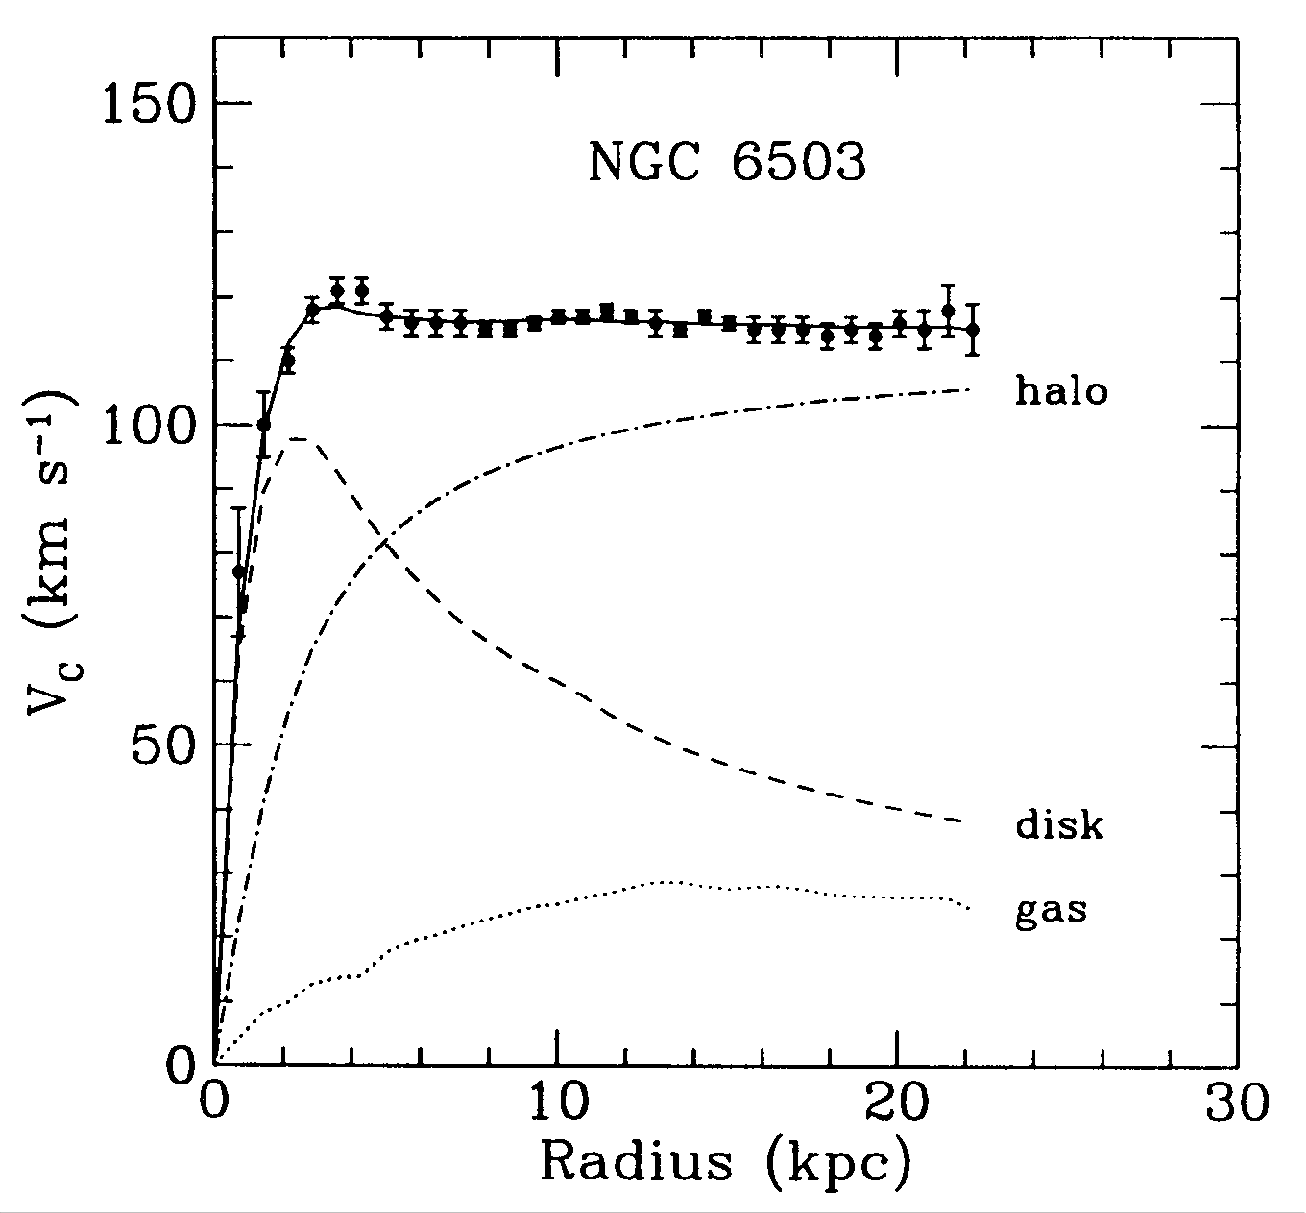
\includegraphics[width=\largefigwidth]{plots/theory/rotationcurve.png}}

  \subfloat[]{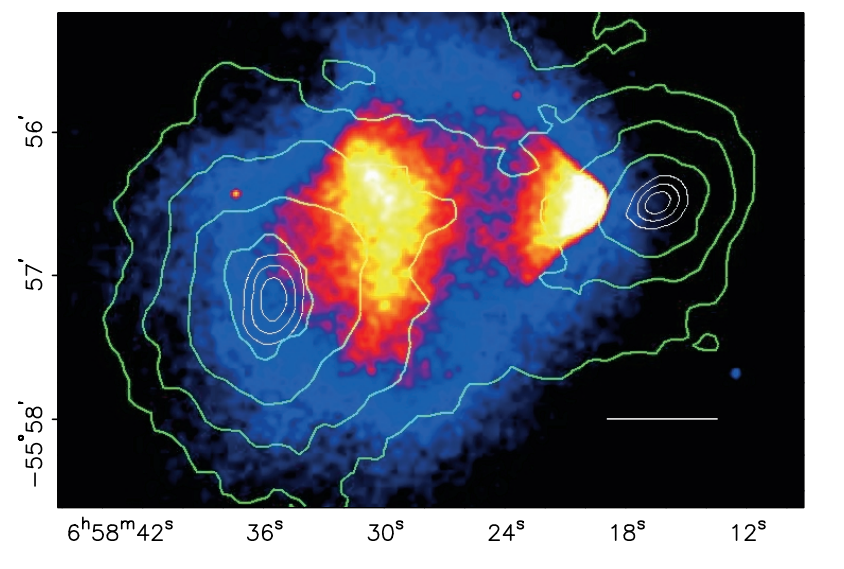
\includegraphics[width=\largefigwidth]{plots/theory/bulletcluster.png}}
  \caption{Evidence for \ac{DM}: (a) Rotation velocity in the galaxy NGC 6503 as a function of distance from the galactic centre~\cite{Freese:2008cz}. (b) The disk and gas components shown are made of visible matter, while the halo component shows the effect of adding an additional \ac{DM} halo to the galaxy. A superposition of X-ray (colour-scale) and gravitational lensing (green contours) images of the bullet cluster of galaxies~\cite{1538-4357-648-2-L109}.}
  \label{fig:dmevidence}
\end{figure}

\section{Searching for dark matter with Higgs bosons}
\label{sec:higgsdm}
%mention collider searches for Dark matter use MET and need associated production
A \ac{SM} 125 \GeV Higgs boson can only decay to invisible final states by first decaying to a pair of \PZ bosons, which then both decay to neutrinos. The branching fraction for this process is less than 1\%~\cite{Heinemeyer:1559921}, so the observation of larger invisible branching ratios of the Higgs boson, \BRinv, would be strong evidence for couplings to \ac{DM}-like particles. Observing decays of Higgs or Higgs-like bosons to \ac{DM} presents an experimental problem in that the final state particles are not visible to the particle detectors used at the Large Hadron Collider (\LHC), such as the Compact Muon Solenoid, CMS~\cite{Chatrchyan:2008aa}, which the data used in this thesis were collected with. Therefore, if a Higgs boson were to be created alone and decay to \ac{DM} there would be no way to observe these decays. Fortunately, several Higgs boson production mechanisms (as described in \SectionRef{sec:higprod} below), lead to additional particles being created with the Higgs boson. By conservation of momentum, the vectorial sum of the momenta of these additional particles transverse to the \LHC beams will be non-zero due to the unobserved particles. This missing transverse momentum, \MET, can therefore be used to identify the presence of \ac{DM} particles in the event. This type of search is referred to as a direct search.

%indirect searches and current Higgs properties limits
Another indication of Higgs boson decays to unseen particles would be a difference between the total decay width of the Higgs boson and the sum of the decay widths of all visible decays. This type of search is referred to as an indirect search. For both direct and indirect searches it is necessary to understand how the Higgs boson is produced and how it decays.

\subsection{Higgs boson production and decay at the LHC}
\label{sec:higprod}
%Detail Higgs production and decays in order to motivate searching for invisible decays in the VBF channel
The LHC (discussed in detail in \SectionRef{sec:lhc}) collides protons at high energies. The results of these collisions are referred to as ``events''. The dominant production mechanisms for Higgs bosons in high energy proton collisions are shown in \FigureRef{fig:smprodfeyn}, and they have the cross-sections shown in \FigureRef{fig:smprod}. It can be seen that \ac{ggH} production, where two gluons fuse via a quark loop to produce a Higgs boson (as shown in \FigureRef{fig:smprodfeyn}a), has the highest cross-section across the full Higgs boson mass range shown. Unfortunately, this production mode normally results in no visible particles in the final state and therefore most \ac{ggH} events cannot be used to search for invisibly decaying Higgs boson. In some \ac{ggH} events there is \ac{QCD} radiation from the initial state particles (\ac{ISR}). Due to asymptotic freedom ~\cite{PhysRevLett.30.1343,PhysRevLett.30.1346} these radiated quarks and gluons each result in a collimated ``jet'' of hadrons in the final state, and thus allow invisibly decaying Higgs boson searches to be performed. However, the visible particles in these events are hard to distinguish from other similar \ac{QCD} background processes with much larger cross-sections, so \ac{ggH} is not the most promising channel for invisibly decaying Higgs boson searches.

The next highest cross-section production process is \ac{VBF}. As can be seen in \FigureRef{fig:smprodfeyn}b, this process involves two incoming quarks both radiating vector bosons which fuse, resulting in a Higgs boson. The two initial quarks form jets in the final state, providing visible particles with which to perform an invisibly decaying Higgs boson search. Furthermore, the lack of a strong force connection (referred to as ``colour connection'') between the two quarks means that the resulting jets have a distinctive topology, being well separated in their angle to the beamline, and also that there is very little other hadronic activity in \ac{VBF} events. This distinctive topology and high cross-section make \ac{VBF} the most sensitive production channel for invisibly decaying Higgs boson searches. For this reason, this thesis will focus on the \ac{VBF} channel.

After \ac{VBF}, \ac{VH} production has the next highest cross-section. \ac{VH} results in a Higgs boson and a vector boson, which decays resulting in visible particles in the final state allowing invisibly decaying Higgs boson searches to be carried out. In the case of leptonic vector boson decays, these final state particles can be relatively easy to identify, resulting in lower backgrounds than in the case of searches in the \ac{VBF} and \ac{ggH} channels. However, the lower cross-section means that the \ac{VH} channel is not as sensitive as \ac{VBF}.

Finally, the fourth highest cross-section Higgs boson production channel is top quark associated production, where the final state consists of two top quarks and a Higgs boson. Whilst the top quarks do decay to visible particles which could be identified, the cross-section for this process is too low, and the backgrounds are too high for an invisibly decaying Higgs boson search to be carried out using the Run 1 \LHC data.

\begin{figure}
    %ggh
  \subfloat[]{
    \begin{fmfgraph*}(150,150)
      \fmfleft{i0,i2,ix,i3,i5}
      \fmfright{o0,o3,o1,o4,o6}
      \fmf{phantom,tension=4/3}{i2,v1,o3}
      \fmf{phantom,tension=4/3}{i3,v2,o4}
      \fmffreeze
      \fmf{gluon,tension=4/3}{i2,v1}
      \fmf{gluon,tension=4/3}{i3,v2}
      \fmf{fermion,tension=0}{v1,v2}
      \fmf{fermion,tension=2/3}{v2,v3,v1}
      \fmf{dashes}{v3,o1}
      \fmflabel{$g$}{i2}
      \fmflabel{$g$}{i3}
      \fmflabel{$H$}{o1}
  \end{fmfgraph*}}    
  %vbf
  \hspace{3.5cm}
  \subfloat[]{
    \begin{fmfgraph*}(150,150)
      \fmfleft{i1,i2}
      \fmfright{o1,o2,o3}
      \fmf{fermion}{i1,v1,o1}
      \fmf{fermion}{i2,v2,o3}
      \fmf{photon,label=$W,,Z$}{v1,v3}
      \fmf{photon,label=$W,,Z$}{v2,v3}
      \fmf{dashes}{v3,o2}
      \fmflabel{$q$}{i1}
      \fmflabel{$q$}{i2}
      \fmflabel{$q$}{o1}
      \fmflabel{$q$}{o3}
      \fmflabel{$H$}{o2}
  \end{fmfgraph*}
  \vspace{.5cm}
}

  \vspace{.5cm}
  
    %Higgstrahlung
  \subfloat[]{
    \begin{fmfgraph*}(150,150)
      \fmfleft{i1,i2}
      \fmfright{o1,o2}
      \fmf{fermion}{i1,v1}
      \fmf{fermion}{v1,i2}
      \fmf{photon,label=$W,,Z$}{v1,v2}
      \fmf{photon}{v2,o1}
      \fmf{dashes}{v2,o2}
      \fmflabel{$q$}{i1}
      \fmflabel{$\bar{q}$}{i2}
      \fmflabel{$W,Z$}{o1}
      \fmflabel{$H$}{o2}
  \end{fmfgraph*}
  \vspace{.5cm}
}
  \hspace{3.5cm}
  %tth
  \subfloat[]{
    \begin{fmfgraph*}(150,150)
      \fmfleft{i0,i1,i4,i5,i6,i2,i3}
      \fmfright{o0,o1,o2,o3,o4}
      \fmf{gluon,tension=3/2}{i1,v1}
      \fmf{gluon,tension=3/2}{i2,v2}
      \fmf{fermion}{o1,v1,v3,v2,o3}
      \fmf{dashes,tension=3/2}{v3,o2}
      \fmflabel{$g$}{i1}
      \fmflabel{$g$}{i2}
      \fmflabel{$\bar{t}$}{o1}
      \fmflabel{$t$}{o3}
      \fmflabel{$H$}{o2}
  \end{fmfgraph*}
}
  
  \caption{Feynman diagrams for the four \ac{SM} Higgs boson production processes with the highest cross-sections: \ac{ggH} (a), \ac{VBF} (b), \ac{VH} (c) and top quark associated production (d).}
  \label{fig:smprodfeyn}
\end{figure}

\begin{figure}
  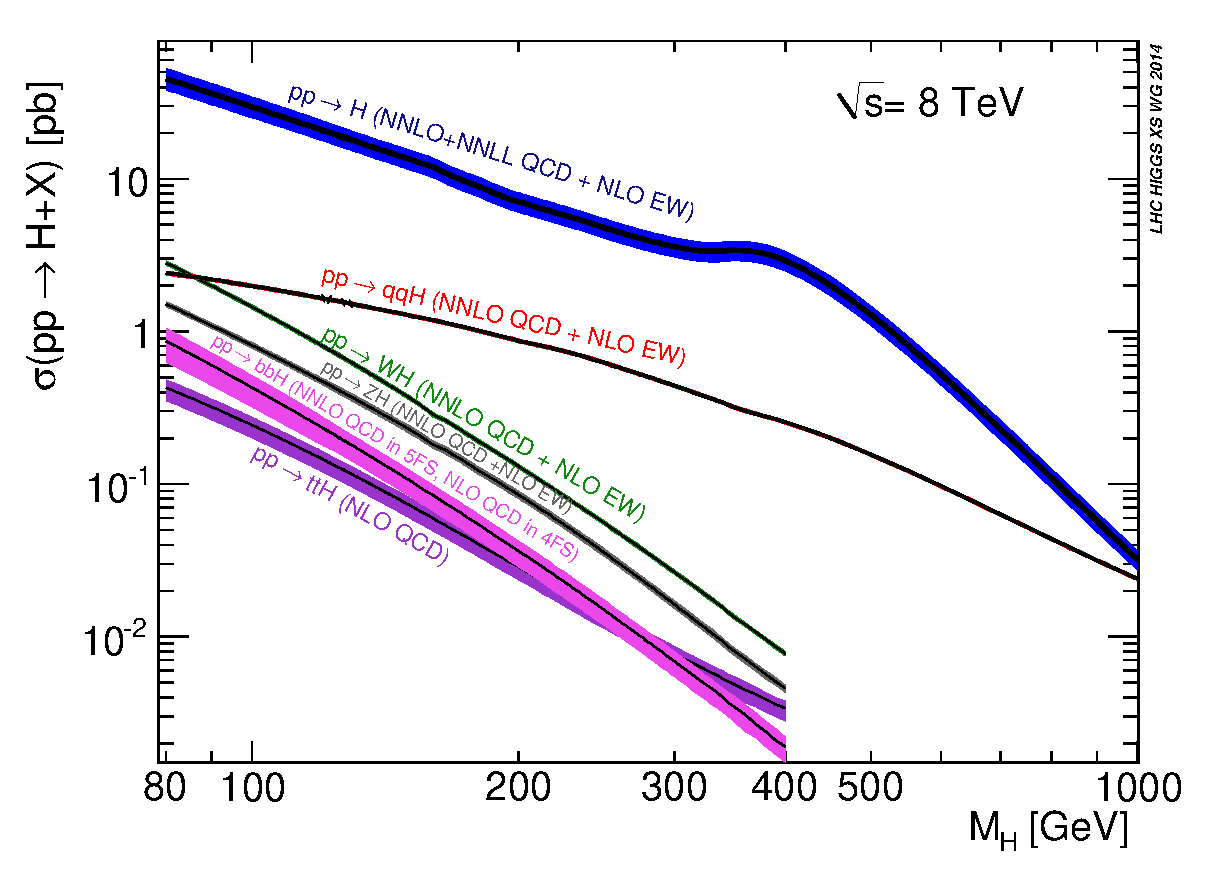
\includegraphics[width=\largefigwidth]{plots/theory/XS_8TeV.eps}
  \caption{Cross-sections for Higgs boson production via the most common production processes at $\sqrt{s}=8 \TeV$ as a function of Higgs boson mass, $m_{H}$~\cite{Heinemeyer:1559921}. The widths of the lines represent the theoretical uncertainties on the cross-section calculation.}
  \label{fig:smprod}
\end{figure}

%talk about SM decays and what SM invisible branching fraction is, direct vs indirect
As mentioned in the introduction to this section, limits can be placed on the Higgs boson's coupling to \ac{DM} by comparing the total decay width of the Higgs boson to the sum of the decay widths for all the visible Higgs boson final states. The branching ratio for the dominant Higgs boson decays as a function of the mass of the Higgs boson can be seen in \FigureRef{fig:smdecay}a. Because a particle's coupling to the Higgs boson is proportional to its mass, the heavier particles have larger branching ratios, with the caveat that particles above half the mass of the Higgs boson, have reduced couplings due to their being created virtually. The \ac{SM} total width of the Higgs boson is shown in \FigureRef{fig:smdecay}b. For a 125 \GeV Higgs boson, the width is only a few \MeV, which is below the current resolution with which it can be measured~\cite{Khachatryan201464}.
Therefore, in order to use the total visible decay width to constrain \BRinv an assumption about the total decay width must be made. 

The current measurements of the branching ratios of the Higgs boson to the 5 most frequent final states can be seen in \FigureRef{fig:smdecaymeasurement}a. The log-likelihood as a function of \BRinv, obtained from these measured branching ratios, assuming the \ac{SM} total Higgs boson decay width, is shown in \FigureRef{fig:smdecaymeasurement}b. It can be seen that whilst the most likely value is approximately zero, values of \BRinv up to $\sim35\%$ are not excluded at the 95\% \ac{CL}. This limit leaves significant parameter space open for \ac{BSM} Higgs boson decays. As the above limit assumes the \ac{SM} Higgs boson total width, it is possible that the branching ratio to invisible final states is much larger, making the case for direct measurements even more compelling. Additional Higgs-like bosons that decay to invisible final states are also not excluded.


\begin{figure}
  \subfloat{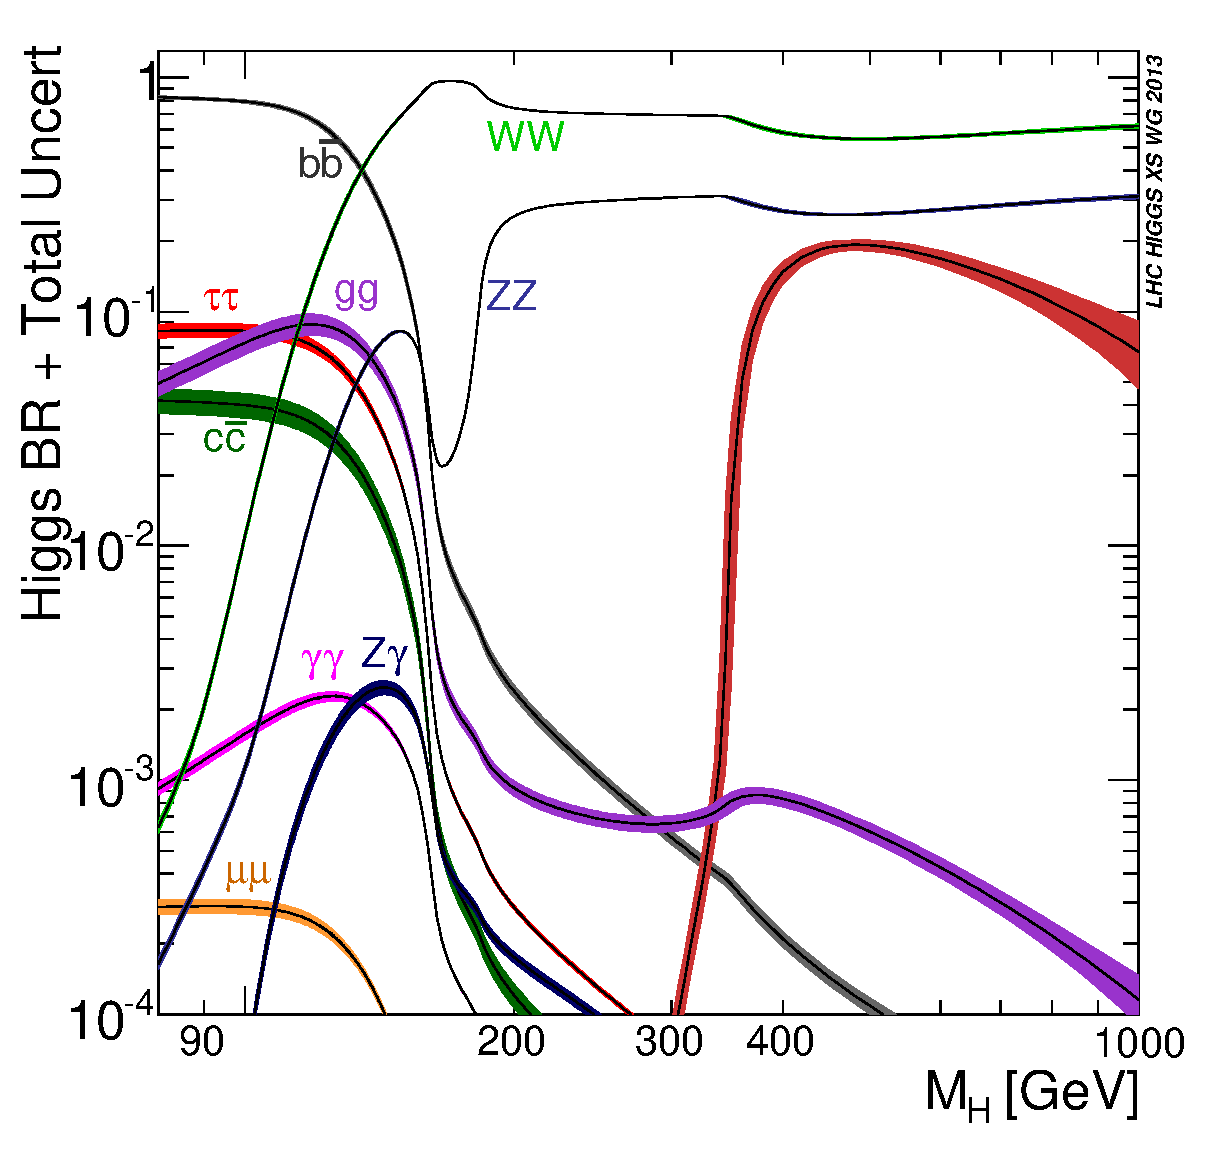
\includegraphics[width=.65\largefigwidth]{plots/theory/Higgs_BR.eps}}
  \subfloat{\includegraphics[width=.65\largefigwidth]{plots/theory/SM_Width-eps-converted-to.pdf}}
  \caption{Branching ratios for the dominant Higgs boson decays as a function of Higgs boson mass with the line widths representing the uncertainties (a), and the \ac{SM} Higgs boson total width, $\Gamma_{H}$, as a function of Higgs boson mass (b)~\cite{Heinemeyer:1559921}.}
  \label{fig:smdecay}
\end{figure}

\begin{figure}
  \subfloat[]{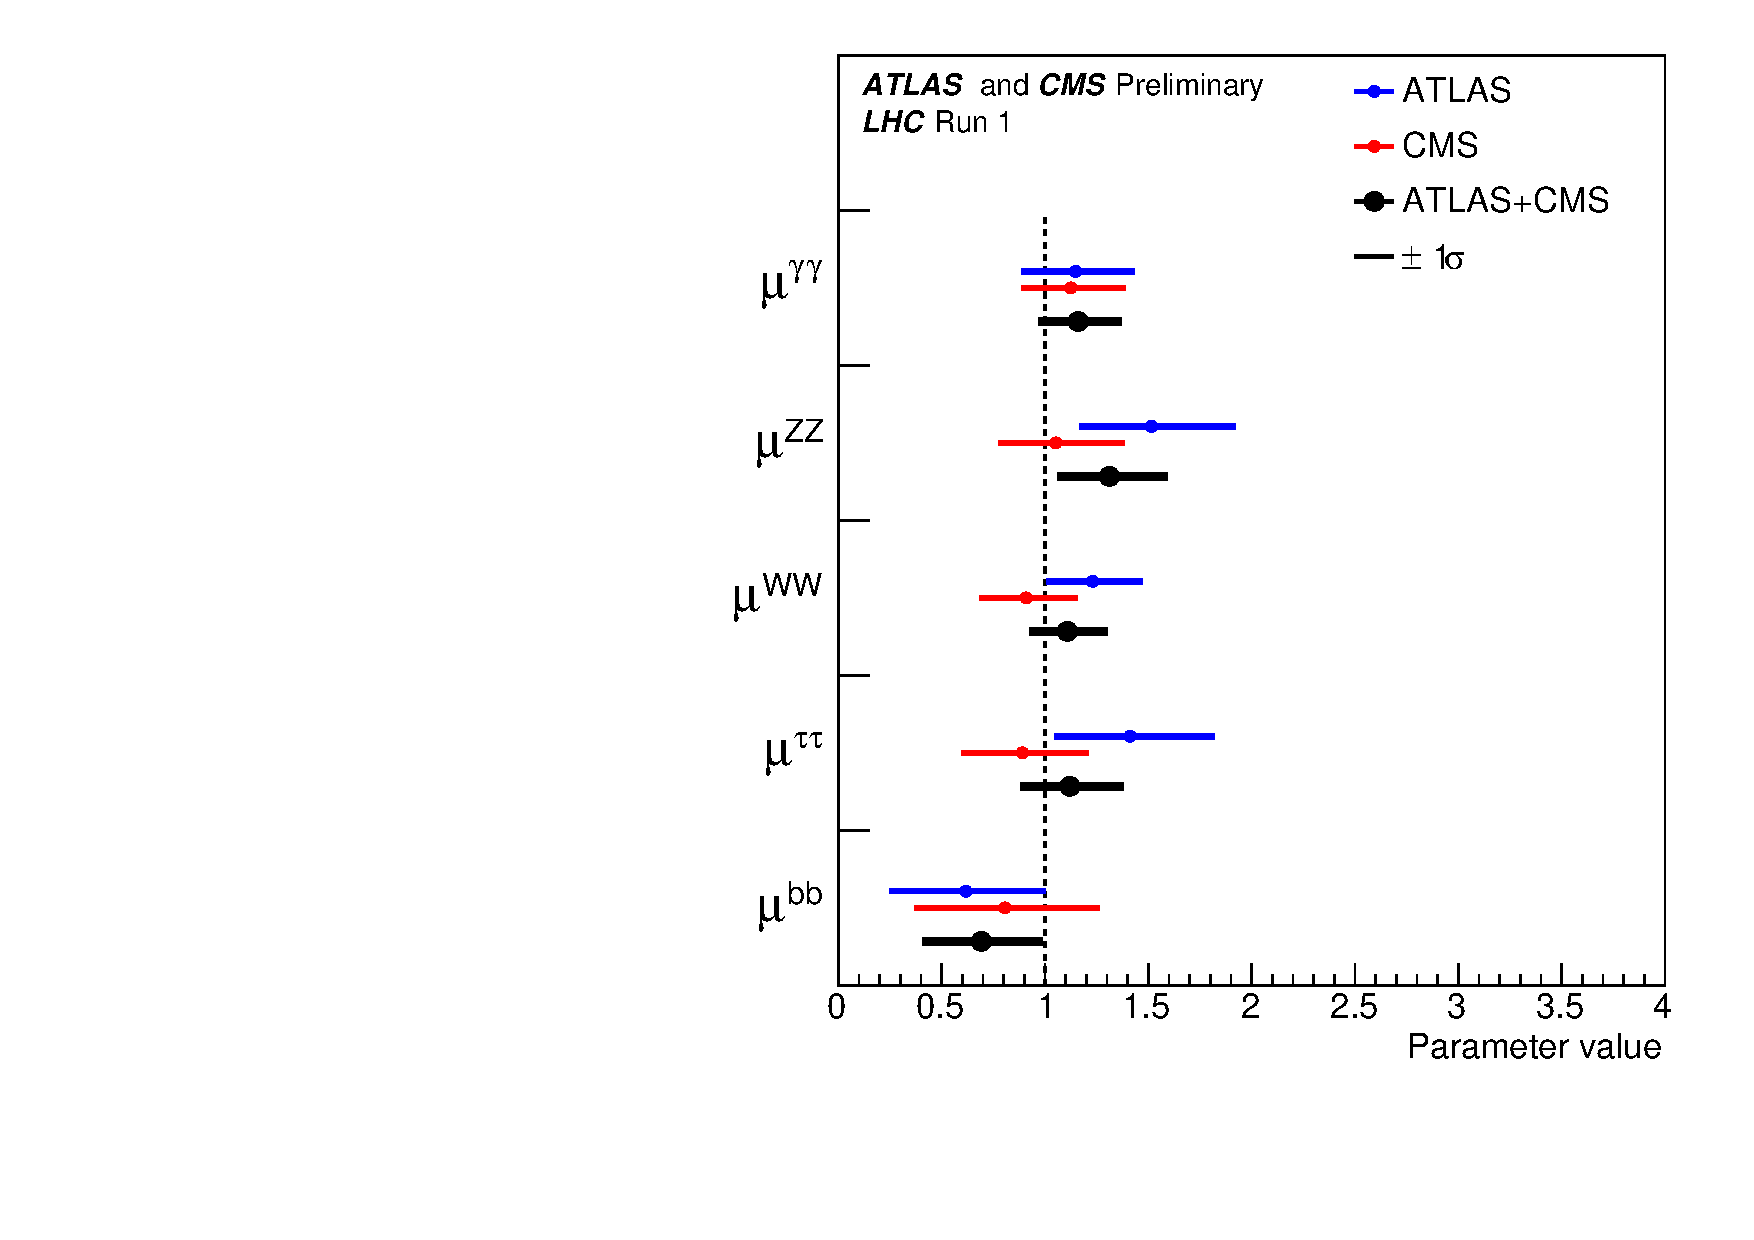
\includegraphics[width=.65\largefigwidth]{plots/theory/smdecaybrlimits.pdf}}
  \subfloat[]{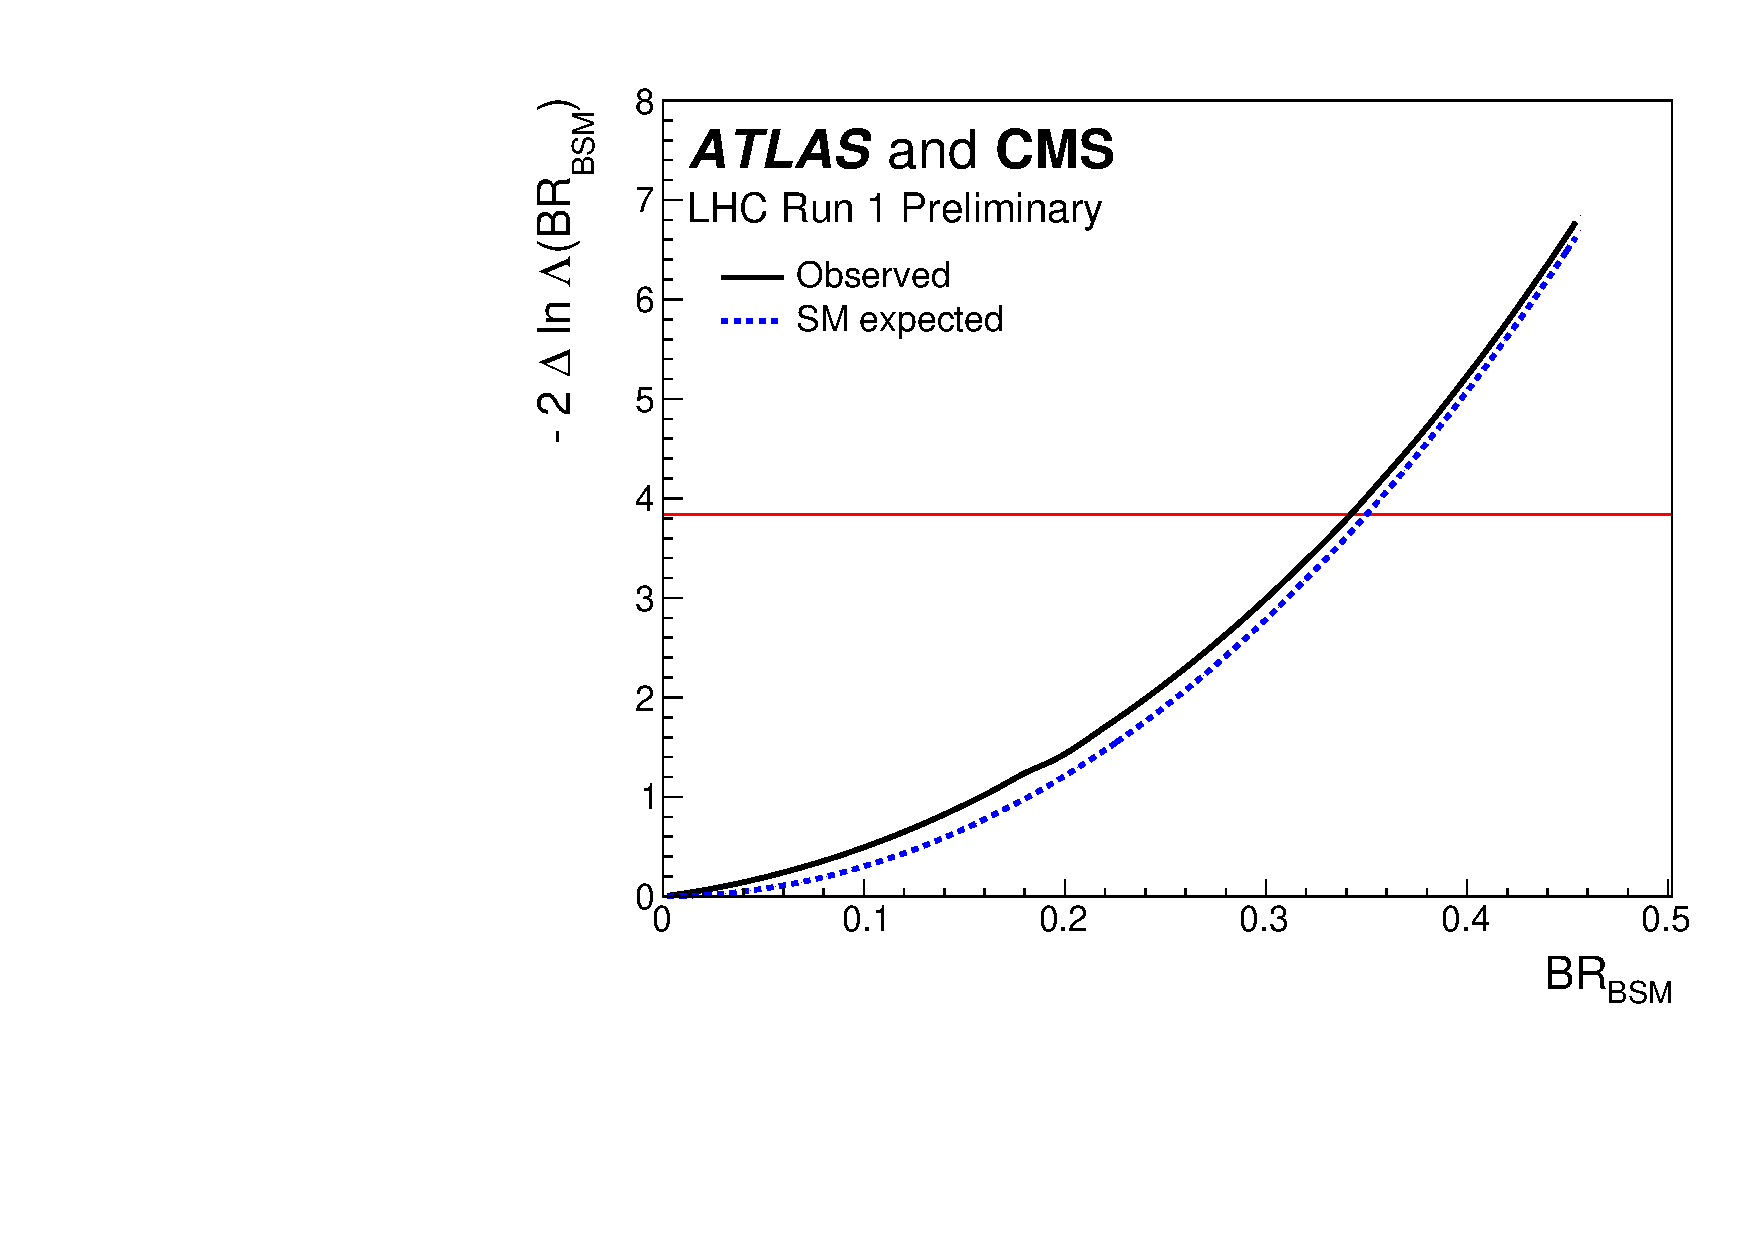
\includegraphics[width=.65\largefigwidth]{plots/theory/smbrbsmlikelihood.pdf}}
  \caption{Best fit results for the decay signal strengths of the five highest branching ratio Higgs boson decays from a combination of CMS and ATLAS~\cite{Aad:1129811} Run 1 data (a). The negative log-likelihood as a function of \BRinv, here denoted $\rm{BR_{BSM}}$ (b)~\cite{CMS-PAS-HIG-15-002}.}
  \label{fig:smdecaymeasurement}
\end{figure}

\subsection{Some extensions of the standard model incorporating dark matter}
\label{sec:DMextensions}
%Introduce theories that are used for pheno work
Whilst current evidence for \ac{DM} is gravitational, the majority of extensions to the \ac{SM} which include \ac{DM} also require other interactions of the proposed \ac{DM} particles. These interactions then allow the particle the \ac{DM} interacts with to act as a ``mediator'' between the \ac{SM} and \ac{DM} particles, for example as in \FigureRef{fig:simplifiedmodelfeynmandiag}a. As all known particles with mass interact with the Higgs boson, it might be expected that \ac{DM}'s interactions with the \ac{SM} are mediated by the Higgs boson or a Higgs-like particle.

\begin{figure}
  \subfloat[]{
    \begin{fmfgraph*}(150,150)
      \fmfleft{i1,i2}
      \fmfright{o1,o4,o2,o5,o3}
      \fmf{fermion}{i1,v1,o1}
      \fmf{fermion}{i2,v2,o3}
      \fmf{photon,label=$W,,Z$,label.side=left}{v1,v3}
      \fmf{photon,label=$W,,Z$,label.side=right}{v2,v3}
      \fmf{dashes,label=$H/A$}{v3,v4}
      \fmf{fermion}{v4,o4}
      \fmf{fermion}{v4,o5}
      \fmflabel{$q$}{i1}
      \fmflabel{$q$}{i2}
      \fmflabel{$q$}{o1}
      \fmflabel{$q$}{o3}
      \fmflabel{$\chi$}{o4}
      \fmflabel{$\chi$}{o5}
  \end{fmfgraph*}
  \vspace{.5cm}
}
  \subfloat[]{
    \begin{fmfgraph*}(150,150)
      \fmfleft{i1,i2}
      \fmfright{o1,o4,o2,o5,o3}
      \fmf{fermion}{i1,v1,o1}
      \fmf{fermion}{i2,v2,o3}
      \fmf{gluon}{v1,v3}
      \fmf{gluon}{v2,v3}
      \fmfdot{v3}
      \fmf{dashes,label=$H/A$}{v3,v4}
      \fmf{fermion}{v4,o4}
      \fmf{fermion}{v4,o5}
      \fmflabel{$q$}{i1}
      \fmflabel{$q$}{i2}
      \fmflabel{$q$}{o1}
      \fmflabel{$q$}{o3}
      \fmflabel{$\chi$}{o4}
      \fmflabel{$\chi$}{o5}
  \end{fmfgraph*}
  \vspace{.5cm}
}
%\vspace{.5cm}
  \subfloat[]{
    \begin{fmfgraph*}(150,150)
      \fmfleft{i1,i2}
      \fmfright{o1,o4,o2,o5,o3}
      \fmf{fermion}{i1,v1,o1}
      \fmf{fermion}{i2,v2,o3}
      \fmf{photon,label=$W,,Z$,label.side=left}{v1,v4}
      \fmf{photon,label=$W,,Z$,label.side=right}{v2,v4}
      \fmfdot{v4}
      \fmf{fermion}{v4,o4}
      \fmf{fermion}{v4,o5}
      \fmflabel{$q$}{i1}
      \fmflabel{$q$}{i2}
      \fmflabel{$q$}{o1}
      \fmflabel{$q$}{o3}
      \fmflabel{$\chi$}{o4}
      \fmflabel{$\chi$}{o5}
  \end{fmfgraph*}
  \vspace{.5cm}
}
  \caption{Feynman diagrams for the dark matter theories considered. (a) \ac{VBF} production of a scalar, $H$, or pseudoscalar $A$ mediator. (b) Gluon based production of an $H$ or $A$ mediator. (c) An effective field theory where the mediator has been replaced by a contact interaction between the vector bosons and a hypothetical \ac{DM} particle.}
  \label{fig:simplifiedmodelfeynmandiag}
\end{figure}

%efts
In \ChapterRef{chap:interp} two classes of these \ac{DM} interaction models are investigated. The first class is \ac{EFT} type models. In these models the mediator is assumed to be much heavier than the momentum transferred through it. This high mass allows the behaviour of the mediator to be replaced by a contact interaction between the \ac{SM} and \ac{DM} particles as shown in \FigureRef{fig:simplifiedmodelfeynmandiag}c. Following the notation in \ReferenceRef{PhysRevD.88.116009}, the particular contact interaction operators considered in this thesis, which each represent a different Lorentz structure for the contact interaction, are:
\begin{align}
  \mathcal{L}_{\rm{D5a}} &=\frac{1}{\Lambda} \left[\bar{\chi}\chi\right] \left[\frac{\PZ_{\mu}\PZ^{\mu}}{2}+\PW_{\mu}^{+}\PW^{-\mu}\right],\\
  \mathcal{L}_{\rm{D5b}} &=\frac{1}{\Lambda} \left[\bar{\chi}\gamma^{5}\chi\right] \left[\frac{\PZ_{\mu}\PZ^{\mu}}{2}+\PW_{\mu}^{+}\PW^{-\mu}\right],\\
  \mathcal{L}_{\rm{D5c}} &=\frac{g_{2}}{\Lambda} \left[\bar{\chi}\sigma^{\mu\nu}\chi\right]\left[\frac{\partial_{\mu}\PZ_{\nu}-\partial_{\nu}\PZ_{\mu}}{cos\theta_{W}} - ig_{2} \left(\PW^{+}_{\mu}W^{-}_{\nu} - \PW^{+}_{\nu}W^{-}_{\mu}\right)\right],\\
  \mathcal{L}_{\rm{D5d}} &=\frac{g_{2}}{\Lambda} \left[\bar{\chi}\sigma_{\mu\nu}\chi\right] \epsilon^{\mu\nu\rho\sigma}\left[\frac{\partial_{\sigma}\PZ_{\rho}-\partial_{\rho}\PZ_{\sigma}}{cos\theta_{W}} - ig_{2} \left(\PW^{+}_{\sigma}W^{-}_{\rho} - \PW^{+}_{\rho}W^{-}_{\sigma}\right)\right],\\
  \mathcal{L}_{\rm{D6a}} &=\frac{g_{2}}{\Lambda^{2}}\partial^{\nu} \left[\bar{\chi}\gamma^{\mu}\chi\right] \left[\frac{\partial_{\mu}\PZ_{\nu}-\partial_{\nu}\PZ_{\mu}}{cos\theta_{W}} - ig_{2} \left(\PW^{+}_{\mu}W^{-}_{\nu} - \PW^{+}_{\nu}W^{-}_{\mu}\right)\right],\\
  \mathcal{L}_{\rm{D6b}} &=\frac{g_{2}}{\Lambda^{2}}\partial_{\nu} \left[\bar{\chi}\gamma_{\mu}\chi\right] \epsilon^{\mu\nu\rho\sigma}\left[\frac{\partial_{\sigma}\PZ_{\rho}-\partial_{\rho}\PZ_{\sigma}}{cos\theta_{W}} - ig_{2} \left(\PW^{+}_{\sigma}W^{-}_{\rho} - \PW^{+}_{\rho}W^{-}_{\sigma}\right)\right],\\
  \mathcal{L}_{\rm{D7a}} &=\frac{1}{\Lambda^{3}} \left[\bar{\chi}\chi\right] \PW^{i,\mu\nu}\PW_{\mu\nu}^{i},\\
  \mathcal{L}_{\rm{D7b}} &=\frac{1}{\Lambda^{3}} \left[\bar{\chi}\gamma^{5}\chi\right] \PW^{i,\mu\nu}\PW_{\mu\nu}^{i},\\
  \mathcal{L}_{\rm{D7c}} &=\frac{1}{\Lambda^{3}} \left[\bar{\chi}\chi\right] \epsilon^{\mu\nu\rho\sigma} \PW^{i}_{\mu\nu}\PW_{\rho\sigma}^{i},\\
  \mathcal{L}_{\rm{D7d}} &=\frac{1}{\Lambda^{3}} \left[\bar{\chi}\gamma^{5}\chi\right] \epsilon^{\mu\nu\rho\sigma} \PW^{i}_{\mu\nu}\PW_{\rho\sigma}^{i},\\
\end{align}
where the \ac{DM} particles, $\chi$, are assumed to be electromagnetically and colour neutral Dirac fermions, and $\PW^{i,\mu\nu}$ is the field strength tensor for the unbroken $SU\left(2\right)_{L}$ gauge bosons. $\Lambda$ is the ``scale'' of the interaction, which is a combination of the mass of the replaced mediator, $M$, and its couplings to both \ac{DM} and the \ac{SM}, $g$, such that $\Lambda\sim M/g^{2}$. Whilst the \ac{EFT} models have the advantage of being simple to interpret, having only one parameter, the validity of the assumption that the momentum transferred through the interaction is much smaller than the mass of the mediator must be checked carefully, especially where the couplings between the mediator and the \ac{DM} are expected to be small. As well as direct searches for invisibly decaying Higgs bosons, several other experimental techniques, including direct dark matter detection are able to set constraints on these models~\cite{ourdmpaper}.%advantages and disadvantages of efts. 

The second class of models are so-called simplified models. In these models an explicit choice of mediator is made, removing the need to make an assumption about the transferred momentum. The specific mediators considered are the 125 \GeV Higgs boson, and scalar and pseudoscalar mediators with heavier masses.

In the case of the 125 \GeV Higgs boson mediator, the following term is added to the Lagrangian:
\begin{equation}
  \mathcal{L}_{H\chi\chi}=-g_{\chi}\left(\bar{\chi}\chi\right)H,
\end{equation}
where the \ac{DM} particles, $\chi$, are again assumed to be Dirac fermions, and $g_{\chi}$ is the Higgs boson coupling to \ac{DM}. As the mediator is very similar to the \ac{SM} Higgs boson all the production mechanisms described in \SectionRef{sec:higprod} are possible, with the most sensitive being \ac{VBF}. If the dark matter mass is below 62.5 \GeV, i.e. it can be created via a real mediator, this interaction leads to an increased invisible decay width of the Higgs boson:
\begin{equation}
  \label{eq:offshellsmhiggs}
  \Gamma\left(H\rightarrow\bar{\chi}\chi\right)=\frac{g_{\chi}^{2}m_{H}}{8\pi}\left(1-\frac{4m_{\chi}^{2}}{m_{H}^{2}}\right),
\end{equation}
where $m_{H}$ and $m_{\chi}$ are the masses of the Higgs boson and the dark matter particle respectively~\cite{ourdmpaper}. For heavier \ac{DM} masses, off-shell production, i.e. through a virtual mediator, is still possible, however there is no invisible branching fraction of the Higgs boson.

For the heavier scalar and pseudoscalar mediators, as well as the free term for the mediator, the terms added to the Lagrangian for the scalar, $H$, and the pseudoscalar, $A$, are:
\begin{align}
  \mathcal{L}_{H}&=-g_{\chi}H\bar{\chi}\chi-\sum_{f}\frac{g_{\rm{V}}y_{f}}{\sqrt{2}}H\bar{f}f\\
  \mathcal{L}_{A}&=-ig_{\chi}A\bar{\chi}\gamma^{5}\chi-\sum_{f}\frac{ig_{\rm{V}}y_{f}}{\sqrt{2}}A\bar{f}\gamma^{5}f,\\
\end{align}
respectively, where $g_{\rm{V}}$ is the coupling of the mediator to visible particles, $f$ are the \ac{SM} fermions, and $y_{f}$ are the \ac{SM} fermion Yukawa couplings~\cite{PhysRevD.91.015017}. The couplings to the \ac{SM} fermions are chosen to be proportional to the \ac{SM} Yukawa couplings so as to avoid constraints from measurements of flavour physics observables~\cite{D'Ambrosio2002155}. Due to the vector boson couplings to the 125 \GeV Higgs boson being compatible with the \ac{SM}, the new mediators do not interact with vector bosons~\cite{CMS-PAS-HIG-15-002}. This lack of vector boson couplings makes \ac{VBF} production, as in \FigureRef{fig:simplifiedmodelfeynmandiag}a, not possible, and leads to the most common production channel for dark matter in association with two jets being the fusion of two gluons as shown in \FigureRef{fig:simplifiedmodelfeynmandiag}b. This gluon fusion occurs, like that seen in the production of the \ac{SM} Higgs boson, through a fermion loop, which is dominated by the top quark due to it having the largest Yukawa coupling.

Again, when the dark matter is less than half the mass of the mediator the mediator will have a non-zero invisible branching ratio. The dark matter production rate will be given by this branching ratio multiplied by the production rate of the mediator. For mediator masses below twice the top quark's mass, and dark matter masses much higher than the $b$ quark's mass, this branching ratio is approximately 100\%. The dark matter production rate is therefore, under the assumption that $g_{V}=g_{\chi}$, proportional to $g_{\chi}^{2}$. For mediator masses larger than twice the top quark's mass, assuming $g_{V}=g_{\chi}$, the branching ratio becomes approximately 41\%~\cite{ourdmpaper} and the production rate remains proportional to $g_{\chi}^{2}$. For dark matter produced through an off-shell mediator the dark matter production rate becomes proportional to $g_{v}^{2}g_{\chi}^{2}$, which simplifies to $g_{\chi}^{4}$ under the assumption of equal \ac{DM} and visible couplings.


\section{Simulation}
\label{sec:sim}
The simulation of \LHC proton-proton collisions can be factorised into several distinct stages, as shown in \FigureRef{fig:factorisation}. The first stage is the hard-scattering of two incoming elements of the proton, called ``partons''. The momentum of each of these partons is sampled from a \ac{PDF}. These \ac{PDF}s give the probability for each incoming parton type to have a certain fraction of the proton's energy at the given hard-scatter energy scale, sometimes referred to as the \ac{QCD} scale. Due to the high energy nature of the hard-scatter, perturbation theory at fixed order can be used for both \ac{QCD} and electroweak interactions at this stage of the simulation. Quantities calculated using the particles which result from the hard-scattering are referred to as ``parton level''.

After the hard-scatter the resulting particles undergo ``parton showering'', which is an iterative process of repeated \ac{QCD} radiation until the particles reach an energy where perturbation theory is no longer valid. After parton showering, particles undergo hadronisation, where colourless hadrons are formed, and allowed to decay. The results of this hadronisation and decay process are four-momentum vectors for each particle which are referred to as the ``generator level'' particles. In most cases the generator level particles are then processed by a \textsc{Geant}~\cite{Agostinelli2003250} 4 based simulation of the CMS detector. For the work described in \ChapterRef{chap:interp} a \textsc{Delphes}~\cite{Favereau2014} based simulation of the CMS detector, which is only approximate, but greatly decreases the computational power needed to process the same number of events.

Several \ac{MC} generators are used to carry out the perturbative hard-scattering calculations. Some, such as \textsc{Pythia}~\cite{Sjöstrand2008852}, are also able to provide the hard-scatter calculation for a wide ranges of processes as well as perform other stages of the factorisation. Others like \textsc{MadGraph}~\cite{Alwall2014} and \textsc{Powheg}~\cite{Nason:2004rx,Frixione:2007vw,Alioli:2010xd} only calculate the hard-scattering component. However, these other generators produce more accurate results for certain processes they have been tuned to, or allow for a larger range of processes to be simulated than the multipurpose generators such as \textsc{Pythia}. In all of the \ac{MC} samples used in this thesis, the results of the hard-scatter are then passed on to \textsc{Pythia} for parton showering and hadronisation.

Finally, some generators, such as MCFM~\cite{PhysRevD.68.094021}, VBFNLO~\cite{Baglio:2014uba,Arnold:2011wj,Arnold20091661}, \textsc{Top++} ~\cite{Czakon20142930} and \textsc{FEWZ}~\cite{PhysRevD.86.094034} are used only to calculate cross-sections very accurately at \ac{NLO} or \ac{NNLO}. These calculations are much more computationally intensive than the lower order calculations above, which renders them unsuitable for generating full \ac{MC} samples with a four vector for each final state particle.

\begin{figure}
  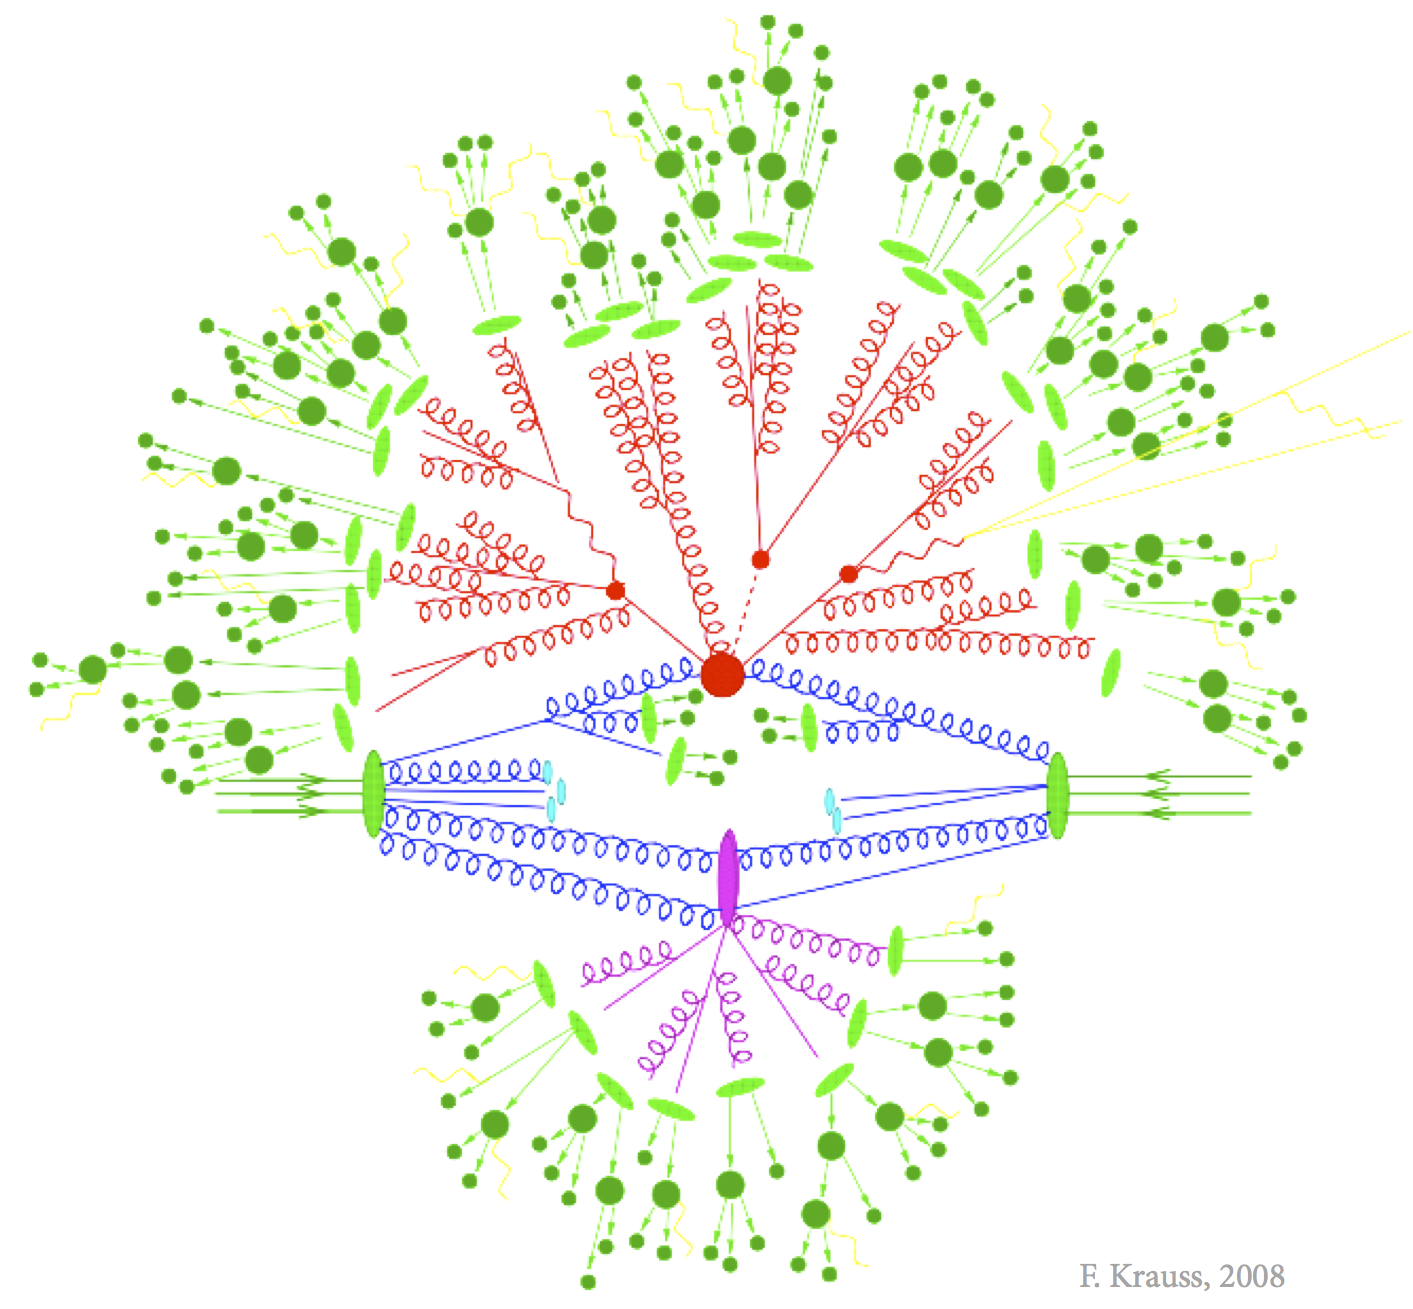
\includegraphics[width=\largefigwidth]{plots/theory/factorisation.png}
  \caption{A schematic diagram of the factorised components of the simulation of proton-proton collisions. First the hard-scatter of two of the incoming partons (shown in blue) is simulated at the centre of the event. The results of this scatter then undergo parton showering (shown in red), followed by hadronisation (shown in green) when the energy of the quarks and gluons is low enough that bound states can be formed~\cite{krauss-diag}.}
  \label{fig:factorisation}
\end{figure}

\section{Statistics of exclusion limits}
\label{sec:stats}
%introduce cls and limit setting
Limits on the parameters of theoretical models are presented throughout this thesis. These limits are set by performing a hypothesis test to discriminate between a null, background physics model only, hypothesis, $b$ and a test hypothesis, the signal process, $s$, plus background model. The particular procedure used is based on the CL$_{S}$ statistic and was developed by the LHC Higgs Combination Group. This procedure is used by both the ATLAS~\cite{Aad:1129811} and CMS experiments~\cite{ATL-PHYS-PUB-2011-011}. 

The procedure starts by defining a likelihood function, $\mathcal{L}$, which quantifies how likely a certain observation is given the expectation under a given hypothesis. $\mathcal{L}$ takes the form:
\begin{equation}
  \label{eq:likelihood}
  \mathcal{L}=\displaystyle\prod_{i}Poisson\left(n_{i}|\nu_{i}\left(\mu,\theta\right)\right)\cdot\prod_{j}Constraint\left(\theta_{j},\bar{\theta}\right),
\end{equation}
where the first term is the contribution from the Poisson probability to observe $n_{i}$ events in each analysis category, $i$, given a predicted number of events from the hypothesis, $\nu_{i}$. $\nu_{i}$ is a function of a signal strength parameter, $\mu$, which in the case of the signal hypothesis being an SM Higgs boson is 1 for the SM and 0 for the background only case, and the ``nuisance paramters,'' $\theta$, which account for the uncertainties on parameters of the signal and background models and any correlations between them. The second term in \EquationRef{eq:likelihood} represents the constraints on the allowed values of these nuisance parameters, with $\bar{\theta}$ being the best estimate of $\theta$ obtained from external measurements. The shape of the constraint function varies depending on the nuisance parameter it represents. For example, uncertainties on the event yield in a category are usually modelled with log-normal constraints, which exclude negative values of the event yield. 

Profile likelihood ratios, q$_{\mu}$, are then calculated, which are defined as:
\begin{equation}
  \label{eq:proflikelihood}
  q_{\mu} = -2 \ln\frac{\mathcal{L}(obs|\mu \cdot s + b,\hat{\theta}_{\mu})}{\mathcal{L}(obs|\hat{\mu} \cdot s + b,\hat{\theta})}\,,
\end{equation}
where $obs$ is the observation, and $\hat{\mu}$ and $\hat{\theta}$ are the values of $\theta$ and $\mu$ where the likelihood is maximised given the constraint $0 \geqslant \hat{\mu} \geqslant \mu$. $\hat{\theta}_{\mu}$ are the values of the nuisance parameters that maximise the likelihood for a given $\mu$. The profile likelihood ratio therefore describes how likely it is to observe a signal strength equal to or higher than $\mu$ compared to the most likely signal strength.

The CL$_{s}$ statistic itself is then defined as:
\begin{equation}
  \label{eq:cls}
  CL_{s} = \frac{P(q_{\mu}\geqslant q_{\mu}^{obs} | \mu \cdot s + b)}{P(q_{\mu}\geqslant q_{\mu}^{obs}|b)}\,,
\end{equation}
Where the probability $P$ of a given $q_{\mu}$ is calculated using the asymptotic limit approximation~\cite{Cowan:2010js}. The region in which a signal strength $\mu \cdot s$ is excluded at the $1 - \alpha$ \ac{CL} is then the region for which CL$_{s}$ is less than or equal to $\alpha$, i.e. when the signal hypothesis is $\alpha$ times less probable than the background.
